
While \ref{eq:dt_chi_k_f_k} and \ref{eq:dt_delta_I_f_I} describe multiphase-flow in a general manner, they do not leverage the topology of the dispersed phase. 
Therefore, in this section, we present a Lagrangian-based model capable of describing the dispersed phase with an arbitrary order of accuracy.

\subsection{Fundamental properties}

At this stage, it is crucial to define some fundamental properties associated to each particle.
Following the strategy of \citet{lhuillier2009rheology,lhuillier1992volume,zaepffel2011modelisation} and \citet[Chapter 2]{morel2015mathematical}
we define the mass, position of center of mass, momentum and total energy of the particle $\alpha$, such as,
\begin{align}
    &m_\alpha(t)
    = \int_{\Omega_\alpha(t)} \rho_2  d\Omega,
    % &&
    &\textbf{x}_\alpha(t)
    = \frac{1}{m_\alpha(t) }\int_{\Omega_\alpha(t)} \rho_2 \textbf{x} d\Omega,\\
    % &&
    &\textbf{p}_\alpha(t) 
    = \int_{\Omega_\alpha(t)} \rho_2 \textbf{u}_2^0 d\Omega,
    % &&
    & m_\alpha E_\alpha(t) 
    = \int_{\Omega_\alpha(t)} \rho_2 [e_2^0 + (u_2^0)^2/2] d\Omega,
    \label{eq:position_and_momentum_def}
\end{align}
respectively. 
Where $\Omega_\alpha$ is the domain occupied by the particle $\alpha$ (see \ref{fig:Scheme}). 
Subsequently, we define the velocity of the particle's center of mass, denoted as $\textbf{u}_\alpha$ which is given by $\textbf{u}_\alpha = \ddt{ \textbf{x}_\alpha}$. 
The derivation of $\ddt {\textbf{x}_\alpha}$ is straightforward but requires some algebra which are detailed in \ref{ap:velocity_definition}. 
The final expression reads,
\begin{equation}
    \textbf{u}_\alpha(t) = \frac{1}{m_\alpha(t)} \left(
        \textbf{p}_\alpha(t)
        +  \int_{\Sigma_\alpha(t)} \rho_2 \textbf{r} (\textbf{u}_I^0 - \textbf{u}_2^0)\cdot \textbf{n}_2 d\Sigma
        \right),
        \label{eq:dt_y_alpha}
\end{equation}
where $\textbf{r}(\textbf{x},t) = \textbf{x} - \textbf{x}_\alpha(t)$. 
In Equation \ref{eq:dt_y_alpha}, it can be observed that the first component of the velocity represents the linear momentum divided by the mass of the particle. 
This corresponds to the mass-averaged velocity over the volume of the particle.
The second term in Equation \ref{eq:dt_y_alpha} arises from the contribution of anisotropic mass transfer across the surface of the particle. 
This mass transfer leads to the motion of the particle's center of mass, thereby contributing to the total velocity.
To illustrate this concept, let us consider a fixed drop with no momentum lying over a very hot plate.
In this scenario, we assume that the plate is sufficiently hot to induce evaporation, specifically on the bottom portion of the drop.
Hence, under the effect of an anisotropic evaporation flux one may expect the second term to be non-negligible.
Consequently, the center of mass of the drop has a non-zero velocity in the opposite direction of the plate, even though the momentum is assumed to be zero.
We can also consider the case of the nucleation of a bubble in water. 
In this case, although the particle momentum is null at all time the center of mass of the particle moves due to the growth of the particle. 
In both cases, we need to take into account the mass transfer term in \ref{eq:dt_y_alpha}, while the first term is negligible. 
Note that \ref{eq:dt_y_alpha} generalized usual expression of the center of mass velocity whom neglect the second term.
In the following, we discard the time dependency notation for all Lagrangian quantities denoted by the subscript $_\alpha$ and also $\Sigma(t)$ and $\Omega_\alpha$.
Nevertheless, the reader must understand that all Lagrangian quantities and integration domains subscribed by $_\alpha$ are time dependent. 

The particle's internal relative motions or the \textit{inner velocity} is given by $\textbf{w}_2^0(\textbf{x},t) = \textbf{u}_2^0(\textbf{x}) - \textbf{u}_\alpha(t)$.
Thus, from its definition in \ref{eq:position_and_momentum_def}, we can rewrite the momentum as follows,
\begin{equation}
    \label{eq:momentum_definition_1}
    \textbf{p}_\alpha
    = m_\alpha \textbf{u}_\alpha
    + \int_{\Omega_\alpha} \rho_2 \textbf{w}_2^0 d\Omega.
\end{equation}
Alternatively, by manipulating \ref{eq:dt_y_alpha}, we obtain,
\begin{equation}
    \textbf{p}_\alpha
    =  m_\alpha \textbf{u}_\alpha
    - \int_{\Sigma_\alpha} \rho_2\textbf{r}(\textbf{u}_I^0 - \textbf{u}_2^0)\cdot \textbf{n}_2 d\Sigma
    \label{eq:momentum_definition}
\end{equation}
Therefore, the momentum of a particle can be seen as a sum of the mean velocity plus the integral of the fluctuation (\ref{eq:momentum_definition_1}), with the latter being equivalent to minus the first moment of mass transfer term (\ref{eq:momentum_definition}).
Indeed, by identification we obtain : $\int_{\Omega_\alpha} \rho_2 \textbf{w}_2^0 d\Omega =\int_{\Sigma_\alpha}  \rho_2\textbf{r} (\textbf{u}_I^0 - \textbf{u}_2^0)\cdot \textbf{n}_2 d\Sigma$. 
The essential aspect of this relation highlighted here is that the internal velocity fluctuations within a fluid particle do not contribute to the total linear momentum $\textbf{p}_\alpha$, as long as the anisotropic mass transfer is negligible.  
Additionally, the total energy $E_\alpha$ can be decomposed following a similar procedure which leads us to, 
\begin{equation*}
    \label{eq:E_alpha_def}
    m_\alpha E_\alpha(t) 
    = m_\alpha e_\alpha 
    + W_\alpha
    + m_\alpha (u_\alpha)^2/2
    % + \textbf{u}_\alpha \cdot \int_{\Omega_\alpha(t)} \rho_2  \textbf{w}_2^0 d\Omega
\end{equation*}
where we introduced the internal kinetic energy : $W_\alpha = \int_{\Omega_\alpha(t)} \rho_2  (w_2^0)^2/2 d\Omega$. 
In that expression mass transfer have been neglected. 
The total energy of a particle is the sum of its internal energy $e_\alpha$, internal kinetic energy $W_\alpha$ and the kinetic energy  due to its own center of mass displacement $u_\alpha^2/2$. 
To gain in understanding, let's express $W_\alpha$ in the case of a solid particle.
The velocity inside a solid particle can be expressed : $\textbf{u}_2^0(\textbf{x}_\alpha + \textbf{r}) = \textbf{u}_\alpha + \textbf{r}\times \bm{\omega}_\alpha$ where $\bm{\omega}_\alpha$ is the angular velocity.  
In this case, $W_\alpha = \bm{\omega}_\alpha\bm{\omega}_\alpha\cdot \mathcal{I}_\alpha$ where $\mathcal{I}_\alpha$ is the inertia matrices of the particle. 
As a matter of facts for solid particles $W_\alpha$ represents the angular kinetic energy for solid particles.
Thus, for particles with fluid internal motion, $W_\alpha$ is just a more general definition of the particle internal kinetic energy. 

\subsection{Conservation laws}
We assign to a particle indexed, $\alpha$, occupying the domain $\Omega_\alpha$ (see \ref{fig:Scheme}) an arbitrary Lagrangian property $q_\alpha$ defined by $q_\alpha  = \intO{ f_2^0(\textbf{x},t) }$.
Similarly, we define $q_{I\alpha} = \intS{ f_I^0(\textbf{x},t) }$ as being an integrated surface property associated to the particle $\alpha$.


To describe the evolution of any arbitrary Lagrangian quantity $q_\alpha$, we need to establish its time derivative.
Since, $q_\alpha$ is an integral quantity with a time-dependent domain of integration, we apply the general Reynolds transport theorem for volume integral (exposed in \ref{ap:math}) to compute its time derivative \citep{morel2015mathematical}.
This yields the following expression :
\begin{equation}
    \ddt  q_\alpha
    = \intO{\left[ \pddt f_2^0 + \div\left(f_2^0\textbf{u}_2^0\right) \right]}\\
    + \intS{ f_2^0 (\textbf{u}_I^0-\textbf{u}_2^0)\cdot \textbf{n}_2 }.
\end{equation}
By substituting the integrand of the first integral on the right-hand side (RHS) with \ref{eq:dt_f_k} we obtain the conservation laws of the quantity $q_\alpha$, namely,  
\begin{equation}
    \ddt  q_\alpha
    = \intO{ s_2^0 }
    + \intS{ \left[
        f_2^0 (\textbf{u}_I^0-\textbf{u}_2^0) 
        + \mathbf{\Phi}_2^0 
        \right] \cdot \textbf{n}_2 },
    \label{eq:dt_q_alpha}
\end{equation}
The first term on the RHS accounts for the total contribution of the source term $s_2^0$ to the particle $\alpha$.
While, The second term on the RHS is the surface integration of the exchange terms, which includes the phase transfer flux $f_2^0 (\textbf{u}_I^0-\textbf{u}_2^0)$ and the diffusive flux $\mathbf{\Phi}_2^0$. 
For clarity, let us consider the specific case of the momentum balance, i.e. when $q_\alpha = \textbf{p}_\alpha$.
In this situation, the first term reads as $\intO{ \rho_2\textbf{g} }$ and represents the total weight acting on the particle $\alpha$. 
Likewise, the second term represents the total source of momentum due to phase transfer, and it is expressed as, $\intS{ \rho_2 \textbf{u}_2^0 (\textbf{u}_I^0-\textbf{u}_2^0)\cdot\textbf{n}_2 }$. 
Lastly, $\intS{ \bm{\sigma}_2^0\cdot\textbf{n}_2 }$ represents the resultant of the hydrodynamic forces acting on the surface of the particle.
It is important to notice that under this form, the exchange terms are expressed as integrals of dispersed phase fields denoted by the subscript $_2$.
Nevertheless, depending on the nature of the dispersed phase, these fields may not always be defined.
For infinitely rigid particles it is indeed the case since, the stress $\bm{\sigma}_2^0$ isn't defined.  
Hence, our objective is to express these exchange terms, in terms of the continuous phase field quantities instead of the dispersed phase field, i.e. in terms of $\mathbf{\Phi}_1^0$ and $\textbf{u}_1^0$ rather than $\mathbf{\Phi}_2^0$ and $\textbf{u}_2^0$. 

To address this issue, let us derive the conservation equation for the integrated surface property $q_{I\alpha}$.
To differentiate time-varying surface integrals within time, we can use the general Leibniz rule (see \ref{eq:Leibnitz}), to derive the following expression :
\begin{equation}
    \ddt  q_{I\alpha}
    = \intS{ \left[
        \pddt f_I^0
        +   \gradI \cdot (\textbf{u}_I^0f_I^0)
    \right]}.
    \label{eq:surface_derivative}
\end{equation}
Substituting the RHS terms of \ref{eq:surface_derivative} using \ref{eq:dt_f_I}, and making use of the surface divergence theorem on closed surfaces (see \ref{eq:surf_div_theorem}), gives,
\begin{equation}
    \ddt  q_{I\alpha}
    = \intS{ 
        s_I^0
    }
    - \intS{ \Jump{
        f_k^0 (\textbf{u}_I^0 - \textbf{u}_k^0)
        + \mathbf{\Phi}_k^0
    }}.
    \label{eq:dt_q_I_alpha}
\end{equation}
This equation can be interpreted as the surface conservation equation for the integrated surface property $f_I$, or as the flux jump condition integrated on a closed surface. 
Notice that $\bm{\Phi}_{I}^0$ isn't present in this balance equation. 
This is due to the fact that as mentioned earlier, only the tangential components of $\bm{\Phi}_{I}^0$ appear inside the surface balance equation, while we perform an integration over a closed surface which is null due to \ref{eq:surf_div_theorem}. 

As discussed above we wish to get rid of $\mathbf{\Phi}_2^0$ in \ref{eq:dt_q_alpha}. To achieve this, we treat the particle's volume and surface as a unified entity and derive a conservation equation for $q_\alpha^\text{tot} = q_\alpha + q_{I\alpha}$. 
This is done by summing \ref{eq:dt_q_alpha} and \ref{eq:dt_q_I_alpha} which leads to, 
\begin{equation}
    \ddt  q_\alpha^\text{tot}
    = 
    \intO{ s_2^0 }
    + \intS{ s_I^0 }
    + \intS{ \left[
        f_1^0 (\textbf{u}_I^0-\textbf{u}_1^0) 
        + \mathbf{\Phi}_1^0 
        \right] \cdot \textbf{n}_2 }. 
    \label{eq:dt_q_alpha_tot}
\end{equation}
This equation is the general form of the linear conservation law of $\chi_2 f_2^0 + \delta_I f_I^0$ for the system consisting of the particle volume $\Omega_\alpha$, and its surface $\Sigma_\alpha$. It is applicable to any particle immersed into a continuous phase following the local conservation,\ref{eq:dt_f_k} and \ref{eq:dt_f_I}.
We refer to this equation as the zeroth-order conservation equation or the linear conservation law for the particle $\alpha$.

Following the same assumption as in \ref{sec:local_eq}, i.e. we consider no mass transfer and weightless interfaces, the Lagrangian  mass, momentum and energy equations for a single particle can be derived using the generic form \ref{eq:dt_q_alpha_tot} and reads as, 
\begin{align}
    \label{eq:dt_m_alpha}
    \ddt m_\alpha
    &= 
    0\\
    \label{eq:dt_p_alpha}
    \ddt (m_\alpha \textbf{u}_\alpha)
    &= 
    m_\alpha\textbf{g}
    +  \intS{\bm{\sigma}_1^0 \cdot \textbf{n}_2}\\
    \label{eq:dt_E_alpha}
    \ddt (m_\alpha E_\alpha + s_\alpha \gamma)
    &= 
    m_\alpha \textbf{u}_\alpha \cdot \textbf{g}
    +\textbf{u}_\alpha \cdot \intS{\bm{\sigma}_1^0 \cdot \textbf{n}_2}   
    +\intS{\textbf{w}_1^0 \cdot \bm{\sigma}_1^0 \cdot  \textbf{n}_2} 
    - \intS{\textbf{q}_2^0 \cdot \textbf{n}_2}
\end{align}
where  $\intS{  \bm{\sigma}_1^0 \cdot \textbf{n}_2 }$ is the resultants of the hydrodynamic force and $\intS{ \textbf{q}_1^0 \cdot \textbf{n}_2 }$ is the resultants of the surface heat flux. 
The second term on the right hands side of the energy equation is the work produced by the mean force and the translational motion of the droplets, while $\intS{\textbf{w}_1^0 \cdot \bm{\sigma}_1^0 \cdot  \textbf{n}_2}$ is the work produced by the local forces and local motion of the fluid at the surface of the particle.
Since we integrated the energy over the particle's volume and its surface, we explicitly made appear the surface energy $\gamma s_\alpha$ within the derivative operator. 
Note that these equations does not explicitly account for inter-particle interactions. 
However, it is possible to include manually such forces by noticing that the surface external stress flux $\bm{\sigma}_1^0$ is the sum of hydrodynamic and particles-particles interaction forces, regardless it is pure contact forces from direct contact or a force mediated through the carrier fluid.
From this consideration it is possible to split every term involving the stress $\bm{\sigma}_1^0$ into two terms representing these contributions. 
Same comments can be made for the heat flux $\textbf{q}_1^0$. 
Although this distinction is important, for purpose of clearly we will stay general, and we will keep the fluxes $\bm{\sigma}_1^0$ and $\textbf{q}_1^0$ as such. 

In the spirit of the energy decomposition exposed in \ref{eq:E_alpha_def} the total energy equation can be split into three equations, one for the center of mass kinetic energy, internal motion and internal kinetic energy, namely,  
\begin{align}
    \label{eq:dt_u2_alpha}
    \frac{1}{2}\ddt (m_\alpha u_\alpha^2)
    &= 
    \textbf{u}_\alpha\cdot
    \textbf{g}m_\alpha
    + 
    \textbf{u}_\alpha\cdot
    \textbf{f}_\alpha,\\
    \label{eq:dt_w2_alpha}
    \ddt (W_\alpha + \gamma s_\alpha)
    &= 
    \intS {\textbf{w}_1^0 \cdot \bm{\sigma}_1^0 \cdot \textbf{n}_2 }
    - \intO{ \bm{\sigma}_2^0 : \grad\textbf{u}_2^0 }
    \\
     \label{eq:dt_e_alpha}
    \ddt (m_\alpha e_\alpha )
    &= 
     \intO{ \bm{\sigma}_2^0 : \grad\textbf{u}_2^0  }
    -  \intS{\textbf{q}_1^0\cdot \textbf{n}_2 } 
\end{align}
respectively. 
Note that in \citet{eq:dt_w2_alpha} the use of \ref{eq:dt_rhoI_uI2} makes appear explicitly the derivative of the surface energy $s_\alpha \gamma$. 
Note that under this form we see that the energy loss in the deformation represented by $W_p$ will be gathered in the surface energy which will in turn act as a source term in the internal kinetic energy motion.
The surface tension plays the role as a spring in the energy balance.   
From this set of equation we can easily see that the rate of dissipation terms $\intS{\bm{\sigma}_2^0 : \grad\textbf{u}_2^0}$ represent an energy sink in the equation of $W_\alpha$ while it is a source term in the internal energy equation. 
As it has been observed in the previous section, this terms convert the energy of internal motion to molecular agitation. 
However, the interplay between the center of mass  kinetic energy and the internal fluctuation is not obvious and has no common term with the heat and internal kinetic energy equation.
In fact, we will see that the transfer between these scales is archived thought the fluid phase pseudo turbulent energy. 


Finally, we would like to highlight that  due to the consideration of closed surface, the diffusive flux $\mathbf{\Phi}_I$, plays no role at all in \ref{eq:dt_q_alpha_tot}.
Therefore, in the case of the linear momentum conservation law, the contribution of the surface tension forces exposed in \ref{eq:surface_tension}, do not contribute to the momentum balance in \ref{eq:dt_p_alpha}.
As a consequence, even in the presence of local Marangoni forces, the resultant of the local surface tension forces cancels out in the linear momentum balance.
This fact has already been demonstrated by \citet{hesla1993note} who showed that the surface tension force does not contribute to the linear and angular momentum balance. 
Here, we have provided the general proof that the interfacial diffusive flux $\mathbf{\Phi}_I^0$, which is present at the local scale according to \ref{eq:dt_f_I}, does not contribute to the zeroth-order conservation law of a particle with a closed surface.
This is therefore applicable to other conservation equations, such as the surface energy balance or the surface mass balance of constituents, where surface diffusive fluxes are also present \citep{bothe2022sharp,manikantan2020surfactant}. 

Nevertheless, it is known that surface tension forces impact the hydrodynamic of droplets and bubbles \citep{kentheswaran2022direct,pesci2018computational}. 
Therefore, if the diffusive flux of surface are not involved in the linear conservation law, it must appear at some point in the momentum description of Lagrangian particles. 
To find out where this contribution arise we shall describe the particle with a higher level of accuracy. 
This is the purpose of the next section. 

\subsection{First order moment equations}

To better describe the local properties within the particles, we now introduce the first moment or the dipole of a particle.
We define the first moment of any properties $f_2^0$ and $f_I^0$ by respectively,
\begin{align}
    &\mathcal{Q}_\alpha 
    = \intO{ \textbf{r} f_2^0 },
    &\text{and}&
    &\mathcal{Q}_{I\alpha}
    = \intS{ \textbf{r} f_I^0 },
    \label{eq:first_moment_definition}
\end{align}
where we recall that $\textbf{r} = \textbf{x} - \textbf{x}_\alpha$ is the distance between any point inside $\Omega_\alpha$ or $\Sigma_\alpha$, to the center of mass of the particle $\alpha$.
It is then possible to differentiate these moments with respect to time in order to obtain their conservation laws.
Indeed, considering \ref{eq:dt_f_k}, \ref{eq:dt_f_I} and applying the Leibniz rule for volume and surface integrals (see \ref{eq:Reynolds} and \ref{eq:Leibnitz} respectively), we can show equally that,
\begin{align}
    \ddt {\mathcal{Q}_\alpha}
    &= \intO{ \left(
        \textbf{r} s_2^0         
        + f_2^0  \textbf{w}_2^0 
        - \mathbf{\Phi}_2^0
    \right) },
    + \intS{ \textbf{r} \left[
        \mathbf{\Phi}_2^0
        + f_2^0 (\textbf{u}_I^0-\textbf{u}_2^0)
    \right]\cdot \textbf{n}_2  } 
    \label{eq:dt_Q_alpha}\\
    \ddt {\mathcal{Q}_{I\alpha}}
    &= \intS{ \left(
        \textbf{r}s_I^0
        + f_I^0 \textbf{w}_I^0
        - \mathbf{\Phi}_{I||}^0
    \right) },
    - \intS{\textbf{r} 
    \Jump{\mathbf{\Phi}_k^0
        + f_k^0 (\textbf{u}_I^0 - \textbf{u}_k^0)
    }
    },
    \label{eq:dt_Q_I_alpha}
\end{align}
where $\textbf{w}_I^0 = \textbf{u}_I^0 - \textbf{u}_\alpha$.
The detailed derivation of \ref{eq:dt_Q_alpha} is provided in \ref{ap:moment_derivative}.
The derivation of \ref{eq:dt_Q_I_alpha} follows a similar procedure. 
% \JL{je n'ai pas relu la derivation detaillee en annexe, ... je te fais confiance. par contre en annexe tu ne derive pas le premier moment interfacial. 
% J'imagine que la derivation est la meme encore faut il le preciser. 
% Egalement j'ai regorganise les elements dans les equations precedentes par signification physique. 
% D'ailleurs il y avait des differences dans les deux equations (la premiere $r S$, la seconde $S r$)... 
% Merci de faire attention a ce genre de detail. 
% J'avoue avoir du mal a comprendre l'interpretation physique de l'integrale de la contrainte dans le volume. 
% Comme on en discutait, par exemple pour une particule solide, celle integrale n'est pas determinee, donc il faudrait la remplacer par quelque chose que l'on connait non ? 
% \tb{Dans le cas ou les contrainte ne sont pas defini les degrées de liberté des particules solid font que cette contrainte ne peux ne pas etre prise en compte la partie symmetrique de cette formule 
% permet justement de remonter a la contrainte dans le cas ou elle ne serait pas defini. dans le cas des particue fluid cela a du sens parcontre c'est les contraintes interne qui s'oppose a la deformations}}
% \JL{
%  Enfin bon a discuter (pas forcement ici). 
%  je pense que c'est un point important. 
% }\tb{cela va etre discuter dans la partie ou on traitre du momentum non ?}
% \JL{
%  Par ailleurs dans quel cas l'integrale des fluctuations $w_2$ est elle nulle ? 
%  pour une particule solide est ce le cas ? 
%  j'imagine que oui ? 
%  J'imagine que tout cela est traite plus tard (dans la derniere section), mais ca me parait crucial de bien expliquer a quoi servent ces termes et dans quel cas ils sont nuls. 
%  \tb{dur a expliquer pour une quantité general }
%  }\JL{
%  Une maniere d'expliciter tout cela pourrait etre de separer j'imagine le premier moment (au moins pour la vitesse) en une partie symmetrique et une partie anti symmetrique pour bien differencier ce qui est lie a la vitesse angulaire et la deformation. 
%  \tb{dans ce cas il faudrait donner l'application du momentum maintenant ce qui change le plan}}
In \ref{eq:dt_Q_alpha}, we recognize the first moment of the source term $s_2^0$, the first moment of the diffusive flux term $\mathbf{\Phi}_2^0\cdot\textbf{n}_2$ and the first moment of phase exchange term, $f_2^0 (\textbf{u}_I^0-\textbf{u}_2^0)\cdot\textbf{n}_2$. 
Additionally, two supplementary terms appear in \ref{eq:dt_Q_alpha}, namely : the integral of the diffusive flux $\mathbf{\Phi}_2^0$, and a term related to the fluctuation of the internal velocity $f_2^0 \textbf{w}_2^0$.
Similar observations can be made for the fist moment of surface equation \ref{eq:dt_Q_I_alpha}, as it shares similarities with \ref{eq:dt_Q_alpha}. 
In particular, it is worth noting the presence of the surface diffusive flux $\mathbf{\Phi}_{I||}^0$ in \ref{eq:dt_Q_I_alpha}.
This term will be further discussed and analyzed in the following. 

For similar reason than the linear conservation equations, we sum \ref{eq:dt_Q_alpha} and \ref{eq:dt_Q_I_alpha} to expresses the conservation equation of the total first moment $\mathcal{Q}_\alpha^\text{tot} = \mathcal{Q}_\alpha + \mathcal{Q}_{I\alpha}$.
This leads to the following expression:
\begin{multline}
    \ddt {\mathcal{Q}_\alpha^\text{tot}}
    = \intO{ \left(
        \textbf{r} s_2^0         
        + f_2^0  \textbf{w}_2^0 
        - \mathbf{\Phi}_2^0
    \right) }
    + \intS{ \left(
        \textbf{r}s_I^0
        + f_I^0 \textbf{w}_I^0
        - \mathbf{\Phi}_{I||}^0
    \right) }
    + \intS{ \textbf{r} \left[
        \mathbf{\Phi}_1^0
        + f_1^0 (\textbf{u}_I^0-\textbf{u}_1^0)
    \right]\cdot \textbf{n}_2  }. 
    \label{eq:dt_Q_alpha_tot}
\end{multline}
Likewise, conservation laws can be derived for an arbitrary $n^{th}$ order moments of volume and surface, i.e. for
\begin{align}
    \mathcal{Q}_\alpha^n
    = \intO{
        \textbf{r}^n
        f_2^0 },
        && \text{and} &&
    \mathcal{Q}_{I\alpha}^n
    = \intS{
        \textbf{r}^n
    f_I^0 },
    \label{eq:Q_n_definition}
\end{align} 
respectively, where $\textbf{r}^n$ is the shorthand for the tensor product $\textbf{r}^n = \underbrace{\textbf{rr}\ldots \textbf{rr}}_{n\text{ times}} $ with $n$ times itself. 
It can be shown that the derivative with time of do not involve any additional terms than in \ref{eq:dt_Q_alpha} and \ref{eq:dt_Q_I_alpha}, but rather just the $n^{th}$ order moments of the already presented terms.
We provide the full derivation of $\ddt{ \mathcal{Q}_\alpha^n}$ in \ref{ap:Moments_equations}.
In short, these higher order moments describe the distributions of the local quantities $f_2^0$ and $f_I^0$ inside the domain $\Omega_\alpha$ and $\Sigma$ respectively.
Consequently, an infinite number of moments would be theoretically necessary to recover the fields of $f_2^0$ and $f_I^0$  within $\Omega_\alpha$ and $\Sigma$. 


% At this stage it is difficult to interpret the physical meaning behind these moments equations. 
% Therefore, to gain in understanding. 
We now discuss the second order moment of mass and first order moment of momentum conservation equations. 
In the following examples, we consider the same hypothesis as in thep previous section. 
Following \ref{eq:Q_n_definition} we define the second-order moment of mass and the first-order moment of momentum as respectively,
\begin{equation}
    \mathcal{M}_\alpha 
    = \intO{ \rho_2 \textbf{r} \textbf{r} }
    \;\;\;\text{and}\;\;\;
    \mathcal{P}_\alpha 
    = \intO{ \rho_2 \textbf{r} \textbf{u}_2^0 }.
    \label{eq:first_moment_of_momentum_def}
\end{equation}
Note that $\mathcal{M}_\alpha$ is analogous to the inertia tensor $\mathcal{I}_\alpha$ in solid mechanics, and they are related through the expression, $\mathcal{I}_\alpha = \text{tr}(\mathcal{M}_\alpha)\textbf{I} - \mathcal{M}_\alpha$.
At constant density the tensor $\mathcal{M}_\alpha$ describes the second moment of the volume distribution around the particle's center of mass.
In order to provide a clearer physical interpretation to the moment of momentum tensor, we decompose $\mathcal{P}_\alpha$ into two distinct part, namely,
$\mathcal{P}_\alpha = \mathcal{S}_\alpha+\mathcal{T}_\alpha$ where $\mathcal{S}_\alpha$ represents the symmetric part and $\mathcal{T}_\alpha$ is the antisymmetric part of $\mathcal{P}_\alpha$.
The tensors $\mathcal{S}_\alpha$ and $\mathcal{T}_\alpha$ correspond respectively to the stretching and angular momentum of the particle $\alpha$. 
The tensor $\mathcal{S}_\alpha$ quantifies how fast and in which direction the particle get elongated or flattened, in other worlds it represents the rate of deformation experienced by the particle.
The tensor $\mathcal{T}_\alpha$ is related to the angular momentum of the particle. 
In this study we use the pseudo vector $\bm{\mu}_\alpha = \int0{ \rho_2 \textbf{r} \times \textbf{u}_2^0 }$ to express this quantity. 
Indeed, both  $\mathcal{T}_\alpha$ and $\bm{\mu}_\alpha$ represent the angular momentum and are related through $(\bm{\mu}_\alpha)_i = \epsilon_{ijk} (\mathcal{P}_\alpha)_{jk}= \epsilon_{ijk} (\mathcal{T}_\alpha)_{jk}$, where $\epsilon$ is the third order alternating unit tensor. 
Lastly, we also introduce the scalar $\mathcal{D}_\alpha = \text{tr}(\mathcal{P}_\alpha) = \frac{1}{3}\int0{ \rho_2 \textbf{r} \cdot \textbf{u}_2^0 }.$, which quantifies the rate at which the particle is being compressed.

Injecting, $f_2 = \rho_2$ in the second-order moment equation derived in \ref{ap:Moments_equations} we obtain :
\begin{equation}
    \ddt {\mathcal{M}_\alpha}=2\mathcal{S}_\alpha. 
    \label{eq:dt_M_alpha}
\end{equation}
which is the general form of the second moment of mass conservation equation. 
From \ref{eq:dt_M_alpha} we deduce that the evolution of the distribution of mass of a particle is solely motivated by the stretching of momentum, denoted by $\mathcal{S}_\alpha$. 
This implies that the angular momentum (not to be confused with the angular velocity) plays no-role in the evolution of the second moment of the mass distribution. 
Note that if the particle has a constant $\mathcal{M}_\alpha$ under change of reference frame, such as for spherical particles where we can write $\mathcal{M}_\alpha= \frac{a^2 m_\alpha}{5} \textbf{I}$, then the stretching of momentum is null $\mathcal{S}_\alpha=0$.
This argument has no restriction on the internal particle motion. 
Additionally, applying the trace operator on both sides of \ref{eq:dt_M_alpha}, yields the interesting relation : $\ddt {\text{tr}(\mathcal{M}_\alpha)}=2\mathcal{D}_\alpha$.
Therefore, we can state that $\text{tr}(\mathcal{M}_\alpha) = \lambda^\alpha_1(t)+\lambda^\alpha_2(t)+\lambda^\alpha_3(t)$, with $\lambda_i^\alpha$ for $i=1,2,3$, being the eigenvalues of $\mathcal{M}_\alpha$.
For unreformable particles it is evident that the eigenvalues are not function of time, therefore $\ddt{ \text{tr}(\mathcal{M}_\alpha)}=0$.  
Consequently, $\mathcal{D}_\alpha$ has the notable property of being null whenever the particle shape remain constant, irrespective of the orientation.
The third invariant of this tensor can be shown to be related to the volume of the particle. 

Now, that we described the shape of the particle through its with the symmetric part of the moment of momentum we might need an equation for the moment of momentum. 
This equation is derived injecting $\mathcal{Q}_\alpha = \mathcal{P}_\alpha$ in \ref{eq:dt_Q_alpha_tot}, it reads, 
\begin{equation}
    \ddt {\mathcal{P}_\alpha}
    = \intO{ \left(
        \rho_2  \textbf{w}_2^0 \textbf{w}_2^0 
        - \bm{\sigma}_2^0
    \right) }
    - \intS{ 
        \gamma \textbf{I}_{||}
    }
    + \intS{ \textbf{r}\bm{\sigma}_1^0\cdot \textbf{n}_2} 
    \label{eq:dt_P_alpha}
\end{equation}
The last term on the right hands side of \ref{eq:dt_P_alpha} represents the first hydrodynamic moment of the force traction on the particle surface.
It is commonly  decomposed into a symmetric and an antisymmetric part defined as, 
\begin{align}
    \label{eq:M_decomposition}
    \mathscr{S}_{\alpha,ij}^*
    &= \frac{1}{2}  \intS{ \left[
        r_i(\sigma_{1,jk}^0 n_k)
        + (\sigma_{1,ik}^0 n_k)r_j
        \right]}
    %     - \frac{\delta_{ij}}{3}\int_{\Sigma_\alpha} \left[
    %         r_l(T_{lk}n_k)
    % \right]d\Sigma
    \\
    \mathscr{L}_{\alpha,ij}
    &= \frac{1}{2}  \intS{ \left[
        r_i(\sigma_{1,jk}^0 n_k)
        - (\sigma_{1,ik}^0 n_k)r_j
    \right]}, \nonumber
\end{align}
respectively. 
It will be shown in \ref{sec:averaged_eq} that $\mathscr{S}_\alpha$ is related to a quantity called the stresslet. 
We introduce the torque vector as $\textbf{t}_\alpha = \intS{ \textbf{r} \times (\bm{\sigma}_1\cdot \textbf{n}_2) }$ which is related to the skew symmetric part of the first moments $t_{\alpha,i} = \epsilon_{ikj} \mathscr{L}_{\alpha,jk}$. 
Each of the other terms appearing in \ref{eq:dt_P_alpha} is discussed in further detail in the following.
 

The conservation equation of the angular momentum $\bm{\mu}_\alpha$ is obtained by taking the double contracted product of \ref{eq:dt_P_alpha} with $\epsilon$, which gives the simple expression :
\begin{equation}
    \ddt\bm{\mu}_\alpha
    =  
    % \textbf{t}_\alpha.
    \intS{ \textbf{r} \times \bm{\sigma}_1\cdot \textbf{n}_2 }
    \label{eq:dt_mu_alpha}
\end{equation}
Notice that every terms on the RHS of \ref{eq:dt_P_alpha} vanish due to their symmetric nature apart from the first hydrodynamic moment $\mathcal{M}_\alpha$.
Particularly, the surface tension terms do not appear in the angular momentum balance, which is consistent with the findings of \citet{hesla1993note}. 
As a consequence, the surface tension has no effect on the angular momentum regardless of the particle's shape. 
In the literature it is common to include the torque due to inter-particular interactions in the angular momentum balance, as it is done in \citet{jackson1997locally} and \citet{zhang1997momentum}.
Therefore, we remind the reader that $\bm{\sigma}_0^1$ contain interaction forces thus $\textbf{t}_\alpha$ includes particles-particles interactions.


Taking the symmetric part of \ref{eq:dt_P_alpha}, yield an equation for the stretching of momentum, which can be written as,
\begin{equation}    
    \ddt{\mathcal{S}_\alpha}
    =  \intO{
        \rho_2\textbf{w}_2^0 \textbf{w}_2^0
        - \bm{\sigma}_2^0}
        - \sigma\intS{\textbf{I}-\textbf{nn}}
        + \frac{1}{2}\intS{(\textbf{r}\bm\sigma_2^0+ \bm\sigma_2^0\textbf{r})\cdot \textbf{n}}
    \label{eq:dt_S_alpha}
\end{equation}
One might immediately recognize that this equation is in facts an extension to Batchelor’s famous result, 
\begin{equation*}
    \intO{\bm{\sigma}_2^0}
    + \intO{\bm{\sigma}_I^0}
    = \frac{1}{2}\intS{(\textbf{r}\bm\sigma_2^0+ \bm\sigma_2^0\textbf{r})\cdot \textbf{n}}
\end{equation*}
% \tb{it is also an extension to dolata recent results for teh first and second moment equation }
which has been used widely in stokes flow theory to express the unknown internal stress within solid particles in terms of surface integral, i.e. the stress let $\intS{(\textbf{r}\bm\sigma_2^0+ \bm\sigma_2^0\textbf{r})\cdot \textbf{n}}$.
This relation is the main tools used to express the bulk stress of a suspension, it eventually leads to the computation of the famous Einstein equivalent viscosity upon having an analytical formula for $\intS{(\textbf{r}\bm\sigma_2^0+ \bm\sigma_2^0\textbf{r})\cdot \textbf{n}}$. 
Therefore, the significant aspect of \ref{eq:dt_S_alpha} is that it can be interpreted as a generalized equation for the integrated stress tensor within the volume of the particle.
This will become particularly relevant when determining the total stress of an inertial suspension as it will be mentioned in \ref{sec:averaged_eq}.
On the right hands side of \ref{eq:dt_S_alpha} we can identify several terms: 
the internal kinetic energy $\intO{\rho_2\textbf{w}_2^0\textbf{w}_2^0 }$; 
the integral of the particle internal stress $\intO{ \bm{\sigma}_2^0
 }$; 
the integral of the surface stress $\intS{ \sigma (\textbf{I}- \textbf{nn}) }$; 
and the stresslet tensor, $\intS{(\textbf{r}\bm\sigma_2^0+ \bm\sigma_2^0\textbf{r})\cdot \textbf{n}}$ introduced earlier.
Based on \ref{eq:dt_M_alpha} we can infer that the evolution of $\mathcal{M}_\alpha$ is driven by the internal kinetic energy and the stresslet.
However, it is being counteracted by surface tension forces and internal stresses which tend to oppose the deformation of the particle. 
Therefore, if the surface tension forces play no role in the linear and angular momentum equation, it does impact the stretching of momentum $\mathcal{S}_\alpha$.
As a consequence, the surface tension force impact the hydrodynamic behavior of a particle solely through its action on $\mathcal{S}_\alpha$, which is related to the shape of a particle through \ref{eq:dt_M_alpha}.
As remarked by \citet{batchelor1970stress}, since the surface tension force oppose the deformation of a particle, it can be understood as an elastic force. 
Which, as it will be shown in \ref{sec:averaged_eq} has a role on the bulk stress of the suspension. 
Additionally, note that \ref{eq:dt_S_alpha} can be seen as a formula to reformulate the integral of the internal stress $\pOavg{\bm{\sigma}}$.
Equally, in \ref{ap:moment_derivative} we show how to derive the higher order moment of momentum equations, which can also be viewed as formulas for the higher moments of the internal particle stress. 
It is interesting to mention that in a recent study of \citet{dolata2021faxen} they use energy method and recover the first two moments of momentum equations hidden into another but equivalent form, valid in the stokes flow regime. 


% Lastly, by taking the trace of \ref{eq:dt_Q_alpha_tot}, directly yields the scalar equation :
% \begin{equation}
%     \ddt {\mathcal{D}_\alpha}
%     = \intO{ \left(
%         \rho_2 \textbf{w}_2^0 \cdot \textbf{w}_2^0
%         - \bm{\sigma}_2^0 : \textbf{I}
%         \right) }
%         - 2 s_\alpha \gamma
%         + \text{tr}(\textbf{M}_\alpha)
%     \label{eq:dt_D_alpha}
% \end{equation}
% which correspond to the isotropic work balance within the particle's volume and surface. 
% As a matter of fact, the rate of compression of a particle, denoted by the scalar $\mathcal{D}_\alpha$ evolves according to : 
% the internal kinetic energy, $\intO{\rho_2 \textbf{w}_2^0 \cdot \textbf{w}_2^0 }$;
% the trace of the integral of the hydrodynamic stresses, $\intO{ \text{tr}(\bm{\sigma}_2^0)}$; 
% the surface energy $\intS{ \gamma }$; 
% and the trace of the hydrodynamic first moment, $\text{tr}(\textbf{M}_\alpha)$.
% To provide a concrete insight of the physical implication of the above equation, 
% % we consider the example of spherical bubbles with time dependent radius $a_\alpha(t)$ and show that from the scalar moment of momentum equation one can recover the Rayleigh-Lamb-Plesset equation. 
% % Indeed, in this situation, the internal velocity can be expressed as, $\textbf{w}_2^0 = \frac{d a_\alpha(t)}{dt} \frac{\textbf{r}}{a_\alpha(t)}$, which makes the scalar moment of momentum equation as, 
% % \begin{equation*}
% %     \frac{3}{5}\rho_2 a_\alpha(t)\frac{d^2 a_\alpha(t)}{dt^2}
% %     = \intO{(\bm{\sigma}_2^0)_{kk}}
% %     - a_\alpha(t)\intS{\textbf{n}\cdot \bm{\sigma}_2^0 \cdot \textbf{n}}
% %     - 2 \gamma s_\alpha
% % \end{equation*}
% % Upon making use of the constitutive law $\bm{\sigma}_k^0 = -p_k \textbf{I} + \mu_k (\grad \textbf{u}_k^0 + (\grad \textbf{u}_k^0)^T) + \zeta_k \div \textbf{u}$ which we will consider true in both phases except that for the carrier fluid $\zeta_1=0$, one obtain, 
% \begin{equation*}
%     (\rho_1 + \frac{1}{5}\rho_2)a_\alpha\frac{d^2 a_\alpha}{dt^2}
%     + \frac{3}{2}\rho_1\left(\frac{d a_\alpha}{dt}\right)^2
%     + (4\mu_1 + 3\zeta_2) \frac{1}{a_\alpha}\frac{d a_\alpha}{dt}
%     = \smallavg{p_1}{\Sigma_\alpha} - \smallavg{\sigma}{\Sigma_\alpha} - \frac{2\gamma}{a_\alpha}
% \end{equation*}
% where,  $\smallavg{p_1}{\Sigma_\alpha}$ and  $\smallavg{\sigma}{\Sigma_\alpha}$ are the surface-averaged external pressure and surface tension coefficient respectively, and $\smallavg{p_2}{\Omega_\alpha}$ represent the volume-averaged internal pressures.
% We indeed recovered the Rayleigh-Lamb-Plesset equation. 
% \tb{Re do the derivation}
%  we examine a single spherical fluid particle of radius $a$, immersed in a steady flow such that $\textbf{u}^0 = 0$ on $\Omega$. 
% In this situation, the stress tensor can be written as $\bm{\sigma}_k = \textbf{I} p_k^0$ for $k = 1, 2$ where $p_k^0$ is the local pressure in the phase $k$. 
% Therefore, applying these considerations to \ref{eq:dt_D_alpha} yields the relation, 
% \begin{equation*}
%     \smallavg{p_2^0}{\Omega_\alpha} 
%     - \smallavg{p_1^0}{\Sigma_\alpha}
%     =
%     \frac{2}{a} s_\alpha \gamma
%     \label{eq:Laplace_law}
% \end{equation*}
% Under this form it is evident that \ref{eq:Laplace_law} represent the well-known Laplace's Law. 
% Additionally, in light of \ref{eq:dt_M_alpha}, the scalar moment of momentum equation can be interpreted as an equilibrium equation for the particle internal mass distribution, or moment of inertia, since $\ddt{\text{tr}(\mathcal{M}_\alpha)} = 2 \mathcal{D}_\alpha$. 
% From this argument and \ref{eq:dt_D_alpha}, one is able to derive the \textit{Rayleigh-Plesset} equation by considering compressible spherical particles with a non-constant particles radius $a_\alpha(t)$ and assuming an internal velocity written as, $\textbf{w}^0_2 = \frac{d a_\alpha(t)}{dt}  \frac{\textbf{r}}{a_\alpha(t)}$. 
% % A demonstration of this derivation can be found in the class of \tb{CITER LE COURS DE Lhuillier}. 
% By the mean of kinetic theory \citet{zhang1994averaged} derived the \textit{Rayleigh-Plesset} equation under an equivalent but averaged form.
% What we demonstrated is that the scalar moment of momentum balance, i.e. \ref{eq:dt_D_alpha} quantify any isotropic dynamical related to a particle. 


\subsection{Spheroidal fluid particles}

Many studies have been conducted to determine the influence of the droplets' deformation on suspension Rheology \citet{goddard1967nonlinear,lhuillier1987phenomenology,maffettone1998equation}.
Most of the authors considered the Rheology of such an emulsion for neutrally buoyant droplets in shearing flow. 
In this work we would to present a first glimps  of the form Rheology of deformable droplets or bubbles with relative motion. 
As a first step to describe the rheology we are interested in the kinematic and dynamic of a single deformable drop. 
In \ref{sec:Exemples} we study the case of 

\subsubsection*{The drop shape}

In this study we consider spheroidal particles described by a conformation tensor that we note $\textbf{C}_\alpha(t)$.  
This tensor is defined such that its eigenvalues are the dimensionless square length of the semi-axis of the spheroid minus one, such that $\textbf{C}_\alpha = (a_1^2/a^2 - 1) \textbf{pp} + (a_2^2 /a^2 - 1) (\textbf{I}-\textbf{pp})$ where $r$ is the radius of the sphere of same volume and \textbf{p} the orientation vector of the particle (see Figure \ref{fig:scheme2}).  
In this way $\textbf{C}_\alpha = 0$ when the particle is spherical and  $\textbf{C}_\alpha + \textbf{I}$ is equivalent to the Cauchy strain tensor well-defined in solid mechanics \citet{mwasame2017macroscopic}. 
In a general coordinate system the point on the surface of the spheroid verify the relation, 
\begin{equation*}
    \textbf{r}\cdot(\textbf{C}_\alpha + \textbf{I})^{-1}\cdot\textbf{r} = a^2,
\end{equation*}
where $^{-1}$ is the inverse operator.  
One can verify that the second order moment of mass of the particles is related to the conformation tensor through, $\textbf{M}_\alpha = \frac{m_\alpha  a^2}{5} (\textbf{C}_\alpha + \textbf{I})$. 
The last property of the of this tensor is that it the constant volume conservation can be obtained by ensuring that $\text{det}(\textbf{C}_\alpha +\textbf{I}) = (a_1a_2^2)^2 /(a^6) = 1$. 
\begin{figure}[h!]
    \centering
    \hfill
    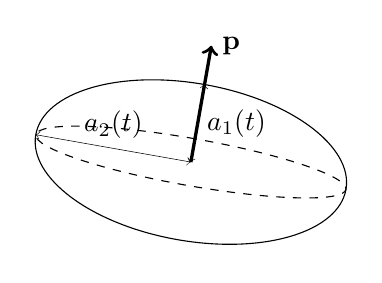
\begin{tikzpicture}[rotate=80]
        \draw(0,0) ellipse (1 cm and 2 cm);
        \draw[dashed](0,0) ellipse (0.3 cm and 2 cm);
        \draw[<->,very thin](0,0) --++ (1,0)node[midway,right]{$a_1(t)$};
        \draw[->,very thick](0,0) --++ (1.5,0)node[right]{$\textbf{p}$};
        \draw[<->,very thin](0,0) --++ (0,2)node[midway,above]{$a_2(t)$};
    \end{tikzpicture}
    \hfill
    \caption{Scheme of an  oblate spheroid oriented along the unit vector \textbf{p} with $a_1(t)$ and $a_2(t)$ the length of the semi axes of the spheroid.}
    \label{fig:scheme2}
\end{figure}


\subsubsection*{The droplet internal velocity}

The internal velocity of a solid elastic particle following a homogeneous linear deformation can be described such as $\textbf{w}_2^0 = \bm\Gamma_\alpha \cdot \textbf{r}$ where we have introduced, $\bm\Gamma_\alpha$, the mean velocity gradient inside the particle, which symmetric part : $\textbf{E}_\alpha$, represents the rate of strain, and skew symmetric part : $\bm\Omega_\alpha$, represents the angular velocity. 
Even through the velocity fields $\textbf{w}_2^0 = \bm\Gamma_\alpha \cdot \textbf{r}$  can apply for liquid deforming droplet, an additional flow is present. 
Indeed, from the solution of the stokes equations we can predict the flow within a spherical isolated drop immersed in an unbounded fluid. 
Especially, we know that an solated droplet in translation exhibit internal motion known as Hill vortexes, see \ref{fig:flowlines} (b). 
For a drop immersed in an unbounded linear flow we can also derive an analytical solution such that $\textbf{w}_2^0 \sim \textbf{rrr}$, see \ref{fig:flowlines} (a). 
Therefore, the droplet's internal velocity fields is constituted with a component accounting for the complex internal motions that does not alter the shape of the drop, and another component that account for the linear deformation of the drop.  
\begin{figure*}
    \centering
    \begin{tikzpicture}
        \node (img3) at (0.6\textwidth,0) {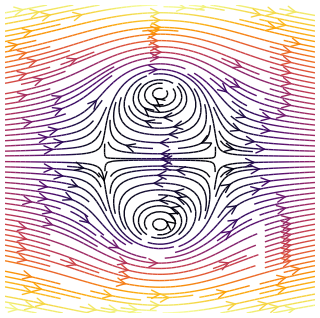
\includegraphics[width=0.3\textwidth,angle=270]{image/Rising_def_Stokes.png}};
        \node (img2) at (0.3\textwidth,0) {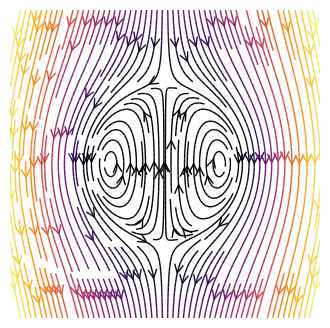
\includegraphics[width=0.3\textwidth]{image/Rising_Stokes.png}};
        % \draw (0.45\textwidth,0)node{$\rightarrow$};
        % \draw (0.45\textwidth,0.4cm)node{$\bm\Gamma_\alpha\cdot \textbf{r}$};
        \node (img1) at (0.0\textwidth,0) {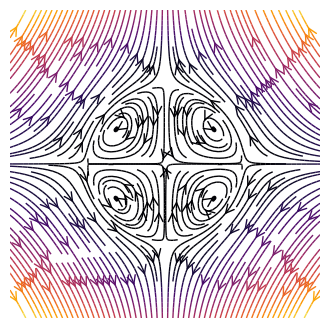
\includegraphics[width=0.3\textwidth]{image/Shear_Stokes.png}};
        \draw (img3.south)node{(c)};
        \draw (img2.south)node{(b)};
        \draw (img1.south)node{(a)};
    \end{tikzpicture}
    \caption{Three examples of steady state flow lines plots of an isolated droplet immersed into a viscous fluid. 
    (a) Rising sphere in uniform stokes flow (analytical solution in \ref{ap:Translating_sphere}). 
    (b) Fixed droplet in extensional flow (analytical solution in \ref{ap:Translating_sphere}).
    (c) Deformed droplet in rising motion (analytical solution of \citet{taylor1964deformation}). }
    \label{fig:flowlines}
\end{figure*}
Consequently, the particle internal velocity might be written, 
\begin{equation}
    \textbf{w}_{2,i}^0(\textbf{x}_\alpha)
    = \bm\Gamma_{\alpha,ik}(t) \cdot \textbf{r}_k
    + \textbf{w}^{s}_2(t,\textbf{r})
    =\bm{\Omega}_{\alpha,ik}\cdot \textbf{r}_k
    + \textbf{E}_{\alpha,ik} \cdot \textbf{r}_k
    + \textbf{w}^{s}_2(t,\textbf{r})
    \label{eq:def_vel}
\end{equation}
Where we introduced the vector $\textbf{w}^{s}_2(t,\textbf{r}) =\textbf{w}^{0}_{2,i}(t,\textbf{r})  - \bm\Gamma_{\alpha,ik}(t) \cdot \textbf{r}_k$ which represents all the internal motions that does not alter the drop's shape. 
Examples of such motions are displayed \ref{fig:flowlines}. 


From now on we consider that the internal velocity $\textbf{w}^{s}_2(t,\textbf{r})$ is not part of the particles unknown, but a function entirely determined by the particle and flow properties such that $\textbf{w}^{s}_2(t,\textbf{r}) =f_\textbf{w}(\textbf{u}_\alpha,\textbf{C}_\alpha,\bm\Gamma_\alpha,\textbf{u}_1,\bm \Gamma_1,\phi_2) $, where $\bm\Gamma_1 = \grad \textbf{u}_1$ and $\textbf{u}_1$ is the mean velocity fields evaluated at the particle position. 
As it is demonstrated in \ref{ap:Translating_sphere} the internal motion of an isolated spherical drop such as the one in \ref{eq:def_vel} might be determined theoretically from the relative motion and flow fields gradient in the limit of low Reynolds number.
We assume that such a relation exist for other regime. 
Consequently, The particle mean velocity gradient $\bm\Gamma_\alpha$ and its conformation tensor $\textbf C_\alpha$ are the only unknown of our problem. 
Therefore, we need to provide two equations, one for $\textbf{C}_\alpha$ and another for $\bm\Gamma_\alpha$. 

\subsubsection*{Kinematic and dynamic of a deformable spheroid}

The evolution of $\textbf{C}_\alpha$ and $\bm\Gamma_\alpha$ will be described by the second moment of mass and first moment of momentum equation.
Consequently, we must reformulate the terms in \ref{eq:dt_M_alpha} and \ref{eq:dt_P_alpha} in terms of $\textbf{C}_\alpha$ and $\bm\Gamma_\alpha$. 
The integrals constitutive of these moments equations can be written, 
\begin{align}
    \intO{(\textbf{rw}_2^0 )_{ij}+ (\textbf{w}_2^0 \textbf{r})_{ij}} 
    = \textbf{C}_{\alpha,ik} \cdot \bm\Gamma_{\alpha,kj}
    +  \bm\Gamma_{\alpha,ki} \cdot \textbf{C}_{\alpha,jk}
    +  \bm\Gamma_{\alpha,ij} + \bm\Gamma_{\alpha,ij}
    \\
    \intO{\rho_2 \textbf{w}_{2,i}^0\textbf{w}_{2,j}^0}
    = \frac{m_\alpha a^2}{5}[
        \bm\Gamma_{\alpha,lj}\bm\Gamma_{\alpha,ki} \textbf{C}_{\alpha,kl} 
        + \bm\Gamma_{\alpha,kj}\bm\Gamma_{\alpha,ki} 
        % + f_\textbf{ww}(\textbf{u}_\alpha,\textbf{C}_\alpha,\bm\Gamma_\alpha,\textbf{u}_1,\bm \Gamma_1,\phi_2)
        + f_\textbf{ww}(\textbf{u}_\alpha,\textbf{C}_\alpha,\bm\Gamma_\alpha,\textbf{u}_1,\bm \Gamma_1,\phi_2)
        ]
    \\
    \label{eq:sigma_2_def}
    \intO{\bm\sigma_{2,ij}^0}
    =
    % -\intO{p_2^0} \textbf{I}_{ij}
    \mu_2 v_\alpha [\bm\Gamma_{\alpha,ij} + \bm\Gamma_{\alpha,ij}
    + f_{\bm{\sigma}}(\textbf{u}_\alpha,\textbf{C}_\alpha,\bm\Gamma_\alpha,\textbf{u}_1,\bm \Gamma_1,\phi_2)]
    % + \textbf{I}_{ij}\intO{p_2^0} 
    \\
    \label{eq:sigma_I_def}
    \intS{\bm\sigma_{I,ij}^0}
    = \frac{2 \gamma v_\alpha }{a} \textbf{I}_{ij} - \frac{4 \gamma v_\alpha }{5 a} \textbf{C}_{\alpha,ij}
    +\mathcal(|\textbf{C}|^2)\\
    \intS{\textbf{r}\bm\sigma_1^0\cdot \textbf{n}_2}
    = 
    \frac{1}{2}\intS{(\textbf{r}\bm\sigma_1^0-\bm\sigma_1^0\textbf{r})\cdot \textbf{n}_2}
    + \frac{1}{2}\intS{(\textbf{r}\bm\sigma_1^0+\bm\sigma_1^0\textbf{r})\cdot \textbf{n}_2}
    % \textbf{M}(\textbf{u}_\alpha,\textbf{C}_\alpha,\bm\Gamma_\alpha,\textbf{u}_1,\bm \Gamma_1,\phi_2)
\end{align}
\tb{mettre sous forme plus simple et expliquer l'osciallater sous forme 1d}
First, as discussed above only the deforming motion contribute to the symmetric part of the moment of momentum, we could therefore express it explicitly in terms of the particle unknown. 
Regarding the first moment of the surface tension, it has been computed analytically carrying a surface integral on the ellipsoidal surface of the droplet. 
Since, the droplets remain spheroidal under small deformation we choose to approximate $\intS{\bm\sigma_I^0}$ with its first order Taylor series in $\textbf{C}_\alpha$ without lost of generality.
Note that our expression of $\intS{\bm\sigma_I^0}$ is in agreement with \citet{lhuillier1987phenomenology} if one account for the slight difference of his definition of the deformation tensor which is half of $\textbf{C}_{\alpha}$. 
% in which our $\textbf{C}_\alpha$ is twice his, in the limit of small \textbf{C}_\alpha.
For the expression of $\intO{\rho_2 \textbf{w}_{2,i}^0\textbf{w}_{2,j}^0}$, $ \intO{\bm\sigma_{2,ij}^0}$ we had to introduce two unknown functions, $f_\textbf{ww}$, $f_{\bm{\sigma}}$, which vanish when $\textbf{w}^s_2 =0$. 
Therefore, these expressions are a sum of a function involving $\bm\Gamma_\alpha$ and an unknown part which depend on the parameters of the problem and need to be closed. 
The expression of $\intO{\rho_2 \textbf{w}_{2,i}^0\textbf{w}_{2,j}^0}$, $ \intO{\bm\sigma_{2,ij}^0}$ and $\intS{\textbf{r}\bm\sigma_1^0\cdot \textbf{n}_2}$ are very problem dependent. 
To provide a clearer example we computed these terms in \ref{ap:Translating_sphere} in the simplified scenario of an isolated droplet in a general linear flow. 

% The most common example is the expression for first moment \textbf{M}, which has been widely investigated in the pure straining situation, an example is given in \ref{ap:Translating_sphere} for spherical drop, and in \citet{raja2010inertial} for slightly deformable droplet in inertial flows. 
% It is important to notice that these functions are dependent of the relative drop-carrier fluid velocity, in such a way that the momentum and first moment of momentum are linked through the function $f_{\textbf{ww}},f_{\bm{\sigma}}$ and $\intS{\textbf{r}\bm\sigma_1^0\cdot \textbf{n}_2}$. 
% Indeed, even if it has been uniquely studied in pure linear flows, the relative motion of a particle might generate a first moment on its surface. 


At this point it wouldn't be wise trying to find an expression for each of these unknown functions in such a generality. 
Instead, we expose the unclosed set of equation of motions for spheroidal particles. 
In addition to the previously exposed equations (mass, momentum and energy equation) this system is constituted of three equations, one for $\textbf{C}_\alpha$ and two equation for the moment of momentum, the symmetric and skew-symmetric moment of momentum. 
% These read, 
% \begin{align*}
%     \ddt \textbf{C}_{\alpha,ij}
%     = \textbf{C}_{\alpha,ik} \cdot \bm\Gamma_{\alpha,kj}
%     +  \bm\Gamma_{\alpha,ki} \cdot \textbf{C}_{\alpha,jk},\\
%     \frac{a^2  m_\alpha}{5} \ddt( \textbf{C}_{ik} \cdot \bm\Gamma_{\alpha,kj}
%     -  \bm\Gamma_{\alpha,ki} \cdot \textbf{C}_{jk})
%     =  \intS{(\textbf{r}\bm\sigma_2^0- \bm\sigma_2^0\textbf{r})\cdot \textbf{n}}\\
%     \frac{m_\alpha a^2}{5}\ddt^2 \textbf{C}_\alpha
%     - \frac{m_\alpha a^2}{5}[
%     \bm\Gamma_{\alpha,lj}\bm\Gamma_{\alpha,ki} \textbf{C}_{\alpha,kl} + f_\textbf{ww}]
%     + \mu_2 v_\alpha [(\bm \Gamma_{p,ij}+\bm \Gamma_{p,ji})
%     + f_{\bm{\sigma}}]\\
%     + \frac{2 \gamma v_\alpha }{a} \textbf{I}_{ij} 
%     - \frac{4 \gamma v_\alpha }{5 a} (\textbf{C}_{ij} - \textbf{I}_{ij})
%     = \intS{(\textbf{r}\bm\sigma_2^0+ \bm\sigma_2^0\textbf{r})\cdot \textbf{n}}
%     % + \textbf{I}_{ij}\intO{p_2^0}
% \end{align*}
% Where we placed the unknown function at the right hands side of these equations. 
Now, we would like to propose a more intuitive interpretation of the mass and momentum equations.
To that end, we make the problem dimensionless by introducing, 
the \textit{Capillary number} $Ca= \frac{\mu_1 U}{\gamma}$, The viscosity ratio $\lambda = \mu_2/\mu_1$, the density ratio $\zeta = \rho_2/\rho_1$ and the Reynolds number $Re = \frac{a U \rho_1}{\mu_1}$, with $U$ as the velocity scale. 
%  such that  $\bm\Gamma_\alpha'  = \frac{a}{U}\bm\Gamma$, and $\tau_a$ the timescale related to the drop shape evolution.
In the low Reynolds regime the first moment of surface traction forces will be proportional to a viscous stress (see \ref{ap:Translating_sphere}), therefore :$\intS{\textbf{r}\bm\sigma_2^0\cdot \textbf{n}} =\mu_1  \tau v_\alpha \intS{\textbf{r}\bm\sigma_2^0\cdot \textbf{n}}^*$, with $\tau$ the inverse timescale of the external solicitation.
The ratio between the external flow scale $\tau$ and the drop timescale $\tau_a$ is noted $\beta$. 
With that in mind, \ref{eq:dt_M_alpha}, \ref{eq:dt_mu_alpha} and \ref{eq:dt_S_alpha} might be written :
\begin{align}
    \label{eq:dt_Cs}
    \beta \ddt \textbf{C}_{\alpha,ij}
    - \textbf{C}_{\alpha,ik} \cdot \bm\Gamma_{\alpha,kj}^*
    - \bm\Gamma_{\alpha,ki}^* \cdot \textbf{C}_{\alpha,jk},
    = 
    \bm\Gamma_{\alpha,ij}^*
    +  \bm\Gamma_{\alpha,ji}^*\\
    Re \zeta \beta \ddt( \textbf{C}_{\alpha,ik} \cdot \bm\Gamma_{\alpha,kj}^*
    -  \bm\Gamma_{\alpha,ki}^* \cdot \textbf{C}_{\alpha,jk}
    + \bm\Gamma_{\alpha,ji} - \bm\Gamma_{\alpha,ij})
    =  \intS{(\textbf{r}\bm\sigma_2^0- \bm\sigma_2^0\textbf{r})\cdot \textbf{n}}^*\\
    \zeta Re \frac{1}{5}  
    \left[
        \frac{1}{2}\beta^2 \ddt^2_* \textbf{C}_\alpha
        - \bm\Gamma_{\alpha,lj}^* \bm\Gamma_{\alpha,ki}^* \textbf{C}_{\alpha,kl}^* 
        - \bm\Gamma_{\alpha,kj}^* \bm\Gamma_{\alpha,ki}^* 
        - f_\textbf{ww}
    \right]\nonumber\\
    + \lambda \left[
        \beta \ddt \textbf{C}_{\alpha,ij}
        -\textbf{C}_{\alpha,ik} \cdot \bm\Gamma_{\alpha,kj}
        - \bm\Gamma_{\alpha,ki}^* \cdot \textbf{C}_{\alpha,jk},
        + f_{\bm{\sigma}}
    \right]\nonumber\\
    - \frac{1}{Ca}\left[
        \frac{4}{5} \textbf{C}_{\alpha,ij}
        +2 \textbf{I}_{ij} 
    \right]
    =
    \frac{1}{2}\intS{(\textbf{r}\bm\sigma_1^0+ \bm\sigma_1^0\textbf{r})\cdot \textbf{n}}^*
    \label{eq:dt2_C}
\end{align}
The second moment of mass \ref{eq:dt_Cs}, is consistent with the equation found by \citet{goddard1967nonlinear} and \citet{lhuillier1987phenomenology}. 
Following, \citet{goddard1967nonlinear}  terminology, the left-hand side of \ref{eq:dt_Cs} is referred as the \textit{convected} derivative of $\textbf{C}^*_\alpha$. 
Therefore, the \textit{convected} derivative of $\textbf{C}_\alpha$ is equal to the rate of strain of the particle. 
The skew-symmetric part of the first moment of momentum \ref{eq:dt2_C}, it is basically the angular momentum balance of a non-spherical object. 
The right-hands side accounting for the external torque contribution. 
The symmetric part however has the form of a non-linear forced harmonic oscillatory equation for the droplet deformation. 
Indeed, the first groups of terms on the left-hand side represent the inertial contribution of the droplet internal fluid. 
It is made of a second order derivative plus non-linear terms in $\bm\Gamma_\alpha$. 
The second groups of terms is internal viscous contribution that arise directly from the definition of the stress \ref{eq:sigma_2_def}. 
It vanishes for small viscosity ration and is linear in the first derivative of $\textbf{C}_\alpha$. 
The last term on the left-hand side is the elastic response from the interface which is negligible for high capillary number $Ca \to \infty$. 
Then on right-hand side of the equation we find the first moment of surface force, $\intS{(\textbf{r}\bm\sigma_1^0+ \bm\sigma_1^0\textbf{r})\cdot \textbf{n}}^*$ which has an unknown expression at this stage. 
\ref{eq:dt2_C} might be regarded as a second order harmonic equation with non-linear contributions. 
However, the unknown function $f_\textbf{ww},\ f_{\bm{\sigma}}$ and $\intS{(\textbf{r}\bm\sigma_1^0+ \bm\sigma_1^0\textbf{r})\cdot \textbf{n}}^*$ are in general function of $\textbf{C}_\alpha$ and its higher derivatives of $\textbf{C}_\alpha$.   
Therefore, at this stage it is impossible to predict the nature of the harmonic regime followed by the droplet. 
To conclude on this matter one must find an expression for all this closure as well as determinate the impact of the non-linear terms.

We now examine the specific case studied by \citet{lamb1924hydrodynamics} where he considered no external contribution around the particle, therefore, $\intS{(\textbf{r}\bm\sigma_1^0+ \bm\sigma_1^0\textbf{r})\cdot \textbf{n}}^* = 0$.
It is found, that the amplitude of the second order harmonic mode of deformation, noted $\epsilon_2$, follows the second order partial differential equations,  
\begin{equation*}
    \ddt^2{\epsilon_2}
    + 2\lambda_2 \ddt \epsilon_2
    + \omega_2^2 \epsilon_2
     = 0,
\end{equation*}
where $\lambda_2$ and $\omega_2$ are the damping and frequency of coefficient defined as, 
\begin{align*}
    \lambda_2 = 5 \frac{\mu_2}{\rho_2a^2},
    && \omega_2 = \sqrt{8 \frac{\mu_2}{\rho_2 a^2}}.
\end{align*}
Where this equation has been obtained in the linear deformation regime for $\epsilon_2 \ll 1$. 
When multiplying \ref{eq:dt2_C} by, $\frac{10}{\zeta Re}$ we indeed find the exact same coefficient $\lambda_2$ and $\omega_2^2$ in front of, $\ddt \textbf{C}_{\alpha,ij}$ and $\textbf{C}_{\alpha,ij}$, respectively. 
In the limit of small $\textbf{C}_\alpha$, only these linear terms remain, therefore consistent with the reference work of \citet{lamb1924hydrodynamics}. 
\ref{eq:dt2_C} is somewhat more general than lamb's solution since it is expressed in an arbitrary reference frame. 
Which will prove to be useful in \ref{sec:Exemples} were we apply ensemble average on these quantities. 
However, with this equation we are able to describe only the second oscillatory mode. 
To study higher order modes one must use higher moment of momentum equations. 

In the past studies, the coupling between translational and oscillating nature of rising bubbles or droplets have been investigated \citet{lalanne2013effect}. 
For an isolated spherical droplet in translation through a stokes or potential flow we know that $
    f_\textbf{ww}
    = \frac{m_\alpha}{140 (\lambda +1)^2}
    (7 \textbf{u}_{\alpha 1} \textbf{u}_{\alpha 1} + \textbf{u}_{\alpha 1}\cdot \textbf{u}_{\alpha 1}\textbf{I})$, 
(see \ref{ap:Translating_sphere}). 
It is reasonable to guess that for a slightly spheroidal droplet in translation the expression might preserve the same form. 
Indeed, a coefficient related to $\textbf{C}_\alpha$ might appear in the expression nevertheless the overall contribution must be still proportional to $\textbf{u}_{\alpha 1} \textbf{u}_{\alpha 1}$. 
Likewise, for an inertial drops, it might be found that 
$\intS{(\textbf{r}\bm\sigma_1^0+ \bm\sigma_1^0\textbf{r})\cdot \textbf{n}}^* \sim A \textbf{u}_{\alpha 1} \textbf{u}_{\alpha 1} + B \textbf{u}_{\alpha 1} \cdot \textbf{u}_{\alpha 1}$ where $A$ and $B$ are constant. 
Indeed, the translational motion a spherical particle at slight inertia induce an overall unbalance stress on the surface of the particle generating a first moment \citet{taylor1964deformation}. 
The point is that the yet unknown closures, will help us bridge translational and drop's straining motions. 
Therefore, injecting these expressions into \ref{eq:dt2_C} would be a first step to accomplish a coupling between oscillating, or deforming motion with translating motion.
This is the subject of the last section. 
Obviously, now that we obtained a general formulation for the dynamic of the droplets' deformation, the most challenging aspect is to find expressions for closure terms. 


% \subsubsection*{The particle internal energy balance.}

% The surface of the particles, and internal kinetic energy can be written in this context as, 
% \begin{align*}
%     \beta \ddt \textbf{C}_{\alpha,ij}
%     - \textbf{C}_{\alpha,ik} \cdot \bm\Gamma_{\alpha,kj}^*
%     - \bm\Gamma_{\alpha,ki}^* \cdot \textbf{C}_{\alpha,jk},
%     = 
%     2\textbf{E}_{\alpha,ij}\\
%     \intO{\rho_2 \textbf{w}_{2,i}^0\textbf{w}_{2,i}^0}
%     = \frac{m_\alpha a^2}{5}[
%         \bm\Gamma_{\alpha,li}\bm\Gamma_{\alpha,ki} \textbf{C}_{\alpha,kl} 
%         + \bm\Gamma_{\alpha,ki}\bm\Gamma_{\alpha,ki} 
%         + f_\textbf{ww}(\textbf{u}_\alpha,\textbf{C}_\alpha,\bm\Gamma_\alpha,\textbf{u}_1,\bm \Gamma_1,\phi_2)
%         ]
%     \\
%     % \label{eq:sigma_2_def}
%     \intO{\bm\sigma_{2,ij}^0:\grad \textbf{u}_2^0}
%     = 2 \mu_2 \intO{\textbf{e}_2^0:\textbf{e}_2^0}
%     = 2\mu_2v_\alpha\left[ \textbf{E}_{\alpha,ij}\textbf{E}_{\alpha,ij}
%     + f_{\textbf{e}}\right]\\
%     % -\intO{p_2^0} \textbf{I}_{ij}
%     \mu_2 v_\alpha [\textbf{E}_{\alpha,ij}
%     + f_{\bm{\sigma}}(\textbf{u}_\alpha,\textbf{C}_\alpha,\bm\Gamma_\alpha,\textbf{u}_1,\bm \Gamma_1,\phi_2)]
%     % + \textbf{I}_{ij}\intO{p_2^0} 
%     \\
%     s_\alpha \gamma
%     = 
%     \frac{3 \gamma v_\alpha }{a}\left[
%         1
%         + \frac{1}{20}\textbf{C}_\alpha:\textbf{C}_\alpha
%     \right]
% \end{align*}

% \begin{equation}
%     \ddt (W_\alpha + \gamma s_\alpha)
%     + \intO{ \bm{\sigma}_2^0 : \grad\textbf{u}_2^0 }
%     =\intS{\textbf{w}_1^0 \cdot \bm{\sigma}_1^0 \cdot \textbf{n}_2} 
% \end{equation}

Hence, we have demonstrated how the first and second moment of momentum and mass equation can be used to describe the second mode oscillatory motion of a spheroidal drop in a Galilean reference frame. 
Therefore, the moment of momentum is a quantity of utmost importance for all kinds of particles with variable shape or volume.
This isn't limited to the momentum distribution, but all kind of properties can be described that way. 
In fact, if one wish to describe the first moment of the distribution of any local quantity $f_2^0$ and $f_I^0$ over the surface or volume of the particle, he must use the first moments' conservation equations. 
As an example, the mean concentration and distribution of surfactants on the bubbles' surface have a significant impact on the mass transfer rate between the dispersed and continuous phases.
In this case first moment of surfactant concentration could be considered here to track the evolution of the surfactant concentration and orientation over the particle surface, which would enable us to compute a better approximation of the drag force coefficient. 

\subsection{From Lagrangian to Eulerian fields}

Up to this point, we have described the dispersed phase within a Lagrangian framework.
However, to be consistent with the Eulerian conservation equations used to describe the continuous phase, we need to extend the Lagrangian equations to an Eulerian models. 
In order to achieve this, we introduce the function $\delta_\alpha$, which is defined as follows, 
\begin{align}
    \delta_\alpha(\textbf{x},t) = \delta(\textbf{x}-\textbf{x}_\alpha(t,\FF)).
    \label{eq:delta_alpha}
\end{align}
where $\delta$ is the Dirac delta function.
Note that we explicitly note $\textbf{x}_\alpha(t,\FF)$ since the posiiton of the particle $\alpha$ is function of time and of the flow configuration $\FF$.
In the sens of generalized functions, the partial time derivative, $\pddt \delta_\alpha(\textbf{x},t,\FF) =  \frac{\partial \textbf{x}_\alpha}{\partial t} \cdot \grad_{\textbf{x}_\alpha} \delta_\alpha$ can be re-written into the following expression, 
\begin{equation}
    \pddt \delta_\alpha
    + \div (\textbf{u}_\alpha  \delta_\alpha)
    =0,
    \label{eq:dt_delta_alpha}
\end{equation}
where we used the identity, $\grad_{\textbf{x}_\alpha} \delta_\alpha = -\grad \delta_\alpha$ and the fact that $\textbf{u}_\alpha(t;\FF)$ is not a function of $\textbf{x}$. 
Additionally, it should be noted that \ref{eq:dt_delta_alpha} is not applicable if changes in topology, such as break up or coalescence events, occur.
In such cases it is possible, as it is done in population balance equations, to include a source term on the RHS of \ref{eq:dt_delta_alpha} to account for particle birth or death. 
Multiplying each Lagrangian quantities by $\delta_\alpha$ yields the \textit{particle field} of a quantity $q_\alpha$, denoted as $q_\alpha(t)\delta_\alpha(\textbf{x},t)$, which is defined throughout space and time.
Likewise, for any derivative of Lagrangian quantities, such as $\ddt q_\alpha$, we define its corresponding Eulerian field by Multiplying $\ddt q_\alpha$ with $\delta_\alpha$ and show that :
\begin{equation}
    \delta_\alpha \ddt q_\alpha
    = \pddt (\delta_\alpha q_\alpha)
    + \div (\delta_\alpha q_\alpha \textbf{u}_\alpha)
    \label{eq:dt_delta_alpha_q_alpha}
\end{equation}
where we have utilized the fact that $q_\alpha(t)$ and $\textbf{u}_\alpha(t)$ are solely functions of time, and we made use of \ref{eq:dt_delta_alpha}.
Additionally, let's consider a volume containing $N$ particles.
We can then define the particle-field of a given quantity $q_\alpha$ as the sum of all the independent field, i.e. $\sum_{\alpha=0}^N \delta_\alpha q_\alpha$.
Notice that \ref{eq:dt_delta_alpha_q_alpha} remains valid for a sum of fields since derivative operators are linear.
To simplify the notations, we consider implicitly the summation over all particles included in $\Omega$ whenever a Lagrangian field denoted by $\delta_\alpha (\ldots)$ is present.

Multiplying \ref{eq:dt_q_alpha_tot} and \ref{eq:dt_Q_alpha_tot} by $\delta_\alpha$, summing over all particles, and by considering \ref{eq:dt_delta_alpha_q_alpha}, it is straightforward to show that,
\begin{equation}
    \pddt (\delta_\alpha  q_\alpha^\text{tot})
    + \div (\delta_\alpha\textbf{u}_\alpha q_\alpha^\text{tot})
    = \delta_\alpha\intO{ s_2^0 }
    + \delta_\alpha\intS{ s_I^0 }
    + \delta_\alpha\intS{ \left[\mathbf{\Phi}_1^0 + f_1^0 (\textbf{u}_I^0-\textbf{u}_1^0) \right] \cdot \textbf{n}_2 },
    \label{eq:dt_dq_alpha_tot}
\end{equation}
\begin{multline}
    \pddt (\delta_\alpha  \mathcal{Q}_\alpha^\text{tot})
    + \div (\delta_\alpha\textbf{u}_\alpha \mathcal{Q}_\alpha^\text{tot})
    = \delta_\alpha\intO{ \left(
        \textbf{r} s_2^0         
        + f_2^0  \textbf{w}_2^0 
        - \mathbf{\Phi}_2^0
    \right) }\\
    + \delta_\alpha\intS{ \left(
        \textbf{r}s_I^0
        + f_I^0 \textbf{w}_I^0
        - \mathbf{\Phi}_{||I}^0
    \right) }
    + \delta_\alpha\intS{ \textbf{r} \left[
        \mathbf{\Phi}_1^0
        + f_1^0 (\textbf{u}_I^0-\textbf{u}_1^0)
    \right]\cdot \textbf{n}_2  }.
    \label{eq:dt_dQ_alpha_tot}
\end{multline}
Similar consideration can be applied to the higher order moments equations derived in \ref{ap:moment_derivative}.

At this stage, we obtained two sets of equations that can be used to describe the dispersed phase. 
The first set of equations is the global conservation laws, i.e. \ref{eq:dt_chi_k_f_k} with for $k=2$ and \ref{eq:dt_delta_I_f_I}. 
The other is the particle-fields equations, such as \ref{eq:dt_dq_alpha_tot} and potentially the higher moments equations.
Therefore, some comments are in order regarding the differences and compatibility of these two sets of equations.
Solving \ref{eq:dt_dq_alpha_tot} ideally provides us with a field $\delta_\alpha(q_\alpha+q_{I\alpha})$ which contains the Lagrangian properties $q_\alpha+q_{I\alpha}$.
Thus, it corresponds to the volume and surface integral of $f_2^0$ and $f_I^0$ on $\Omega_\alpha$ and $\Sigma_\alpha$ respectively.
While, in \ref{eq:dt_chi_k_f_k} we solve the equation for the complete field $f_2^0$ defined inside the domains $\Omega_\alpha$.  
Thus, from  \ref{eq:dt_f_k} to \ref{eq:avg_dt_dq_alpha_tot} we lose the detailed description of $f_2^0$ within the particles' domain.
Indeed, with \ref{eq:avg_dt_dq_alpha_tot}, we recover solely the integrated value of $f_2^0$ over the particles' volume and surface. 
Therefore, \ref{eq:dt_dq_alpha_tot} can be though as averaged equations of \ref{eq:dt_chi_k_f_k} and \ref{eq:dt_delta_I_f_I} since we recover only the integrated properties of each particle. 
It is important to understand that in this sense, the passage from \ref{eq:dt_chi_k_f_k} and \ref{eq:dt_delta_I_f_I} to \ref{eq:dt_dq_alpha_tot} is an average operation carried out on the particles' volume and surface.
Likewise, \ref{eq:dt_dQ_alpha_tot} is an equation for the first moment of the distribution of $f_2^0$ and $f_I^0$ within the particle's volume and surface.

% Note that this is different to the usual averaged technics that refer to the ones used to derive the classic averaged models such as in \citet{jackson1997locally} and \citet{zhang1994averaged}.
% which are the subject of the following section. 
